\documentclass{article}
\usepackage{graphicx}

\begin{document}

\title{DRC-Hubo Perception Computer}
\author{Daniel M. Lofaro}
\date{2013-03-04}
%\maketitle

\begin{center}
\Large DRC-Hubo Perception Computer\\
\large
Daniel M. Lofaro\\
2013-03-04\\
\end{center}
\normalsize
%\begin{abstract}
This document gives the recommendations for the perception computer size, power, and form factor.
In addition options that were not chosen to be persued are shown.
%\end{abstract}

\section{Recommended Configuration}
\subsection{Overview}
The keypoints about the computer chosen for this recomendation is that:
\begin{itemize}
\item The CPU processing power is addiquite
\item The GPU power is addiquite
\item It uses its own powersource and thus does not need to be powered off of DRC-Hubo's battery
\item The system is modded to run with full GPU functionality when on battery (not typical for laptops).
\end{itemize}

The above reasons are why I recomend the comptuer configuration listed below.


\subsection{Computational and Electronic Atrobutes}
\begin{itemize}
\item Brand: System 76
\item Model: Bonobo Extreme -\textit{https://www.system76.com/laptops/model/bonx6}
\item Processor: 3rd Generation Intel Core i7-3740QM Processor ( 2.70GHz 6MB L3 Cache - 4 Cores plus Hyperthreading ) 
\item Graphics: nVidia GeForce GTX 680M with 4 GB GDDR5 Memory and 1344 CUDA Cores
\item Memory: 32 GB Dual Channel DDR3 SDRAM at 1600MHz - 4 X 8 GB
\item Storage: 180 GB Intel 520 Series SATA III 6 Gb/s Solid State Disk Drive
\item Networking: Gigabit LAN (10/100/1000), WiFi
\item Battery: Extra 89.20 WH 8 Cell Smart Li-ION Battery (3.5 Hour Typical Use)
\item Charger: Full Range AC-in 100~240V, 50~60Hz, 90W AC Adapter, DC output 19V, 4.74A
\end{itemize}

\subsection{Physical Attrobutes}
\begin{itemize}
\item 16.5" x 11.54" x 1.55~1.96" (WxDxH)
\item 42.0 cm x 29.5 cm x 4.0~5.0cm (WxDxH)
\item 8.60 lbs. (3.90 kg.)
\end{itemize}

\subsection{System 76 Bonobo Extreme - Image}
\begin{center}
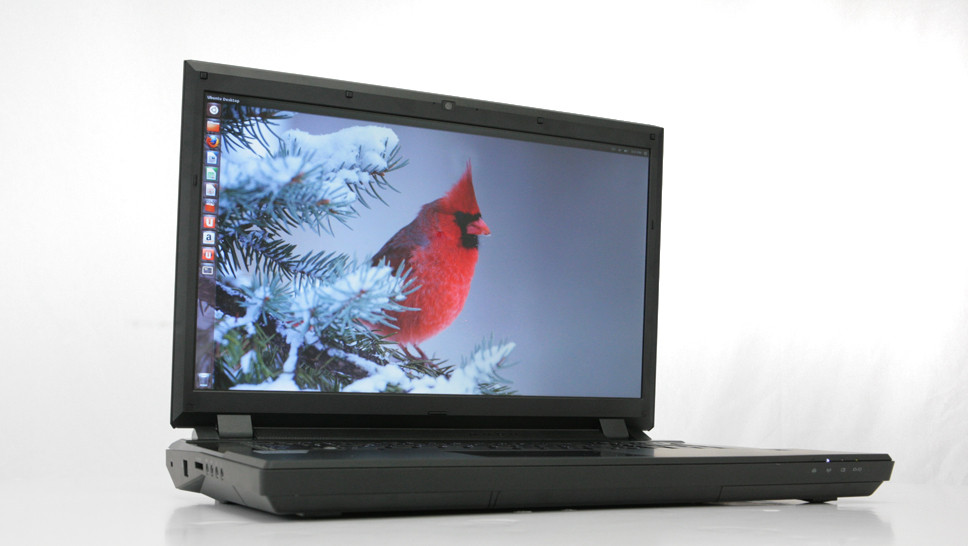
\includegraphics[width=0.75\columnwidth]{./pix/system76.jpg}
\end{center}


\section{Other Non-Recommended Options}
\subsection{PCIe-104 Comptuer with Adaptor}
We could get a PCIe-104 form facor computer with an nVidia graphics card attached (see Sec~\ref{sec:pcie-op}).  
The problem with this option is that there are no PCIe-104 nVidia cards avaliable.
We would have to procure an adaptor card for PCIe-104 socket to normal PCIe (see Sec~\ref{sec:pcie-ad}).

\subsection{PCIe-104 SBC Options}\label{sec:pcie-op}
\subsubsection{Beckhoff - CB4055}
\begin{itemize}
\item CPU: 2.5Ghz i7
\item Max Memory: 4 Gb
\item Power: 5V (Watt not listed)
\item Form Factor: PC-104 - 116 mm x 24 mm x 96 mm
\end{itemize}

\subsubsection{Advanced Digital Logic -ADLQM67PC}
\begin{itemize}
\item CPU: 3.0Ghz i7
\item Max Memory: 8 Gb
\item Power: 5V , 12V, 5V Suspend (Watt not listed)
\item Form Factor: 4.5” x 3.8” (115mm x 96mm) PCI/104-Express v1.0a
\end{itemize}

There are others as well.  One concern is that my trusted company (Advantech) does not sell i7 PCIe-104 SBCs

\subsubsection{PCIe-104 to PCIe Adaptor Card}
In order to a PCIe-104 card with a normal graphics card with CUDA enabled we need 
\begin{itemize}
\item An adaptor
\item External power
\end{itemize}

The adaptor can be something like the \textit{Connect Tech Inc.} PCIe/104 (PCI/104-Express) to PCI Express Adapter:

\begin{center}
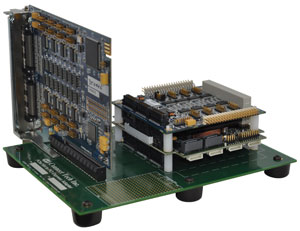
\includegraphics[width=0.75\columnwidth]{./pix/ADG021_web.jpg}\\
URL: \textit{http://www.connecttech.com/sub/products/PCI104\_Express\_PCIe\_B\_Adapter.asp}
\end{center}

\subsection{Use Normal Laptop with ExpressCard PCIe Adaptor}
This option says to use a ExpressCard Adaptor to connect a typical PCIe video card to a laptop computer.
The positive sides of this would be:
\begin{itemize}
\item We can use any PCIe graphics card we want
\item We can use any laptop with a ExpressCard slot that we want
\item This is proven to work in Windows by \textit{Gamers}
\end{itemmize}

The downsides of this option are:
\begin{itemize}
\item We need external power for the graphics card
\item Linux support for the card is not fully tested
\end{itemize}

I am currently in the middle of testing using the PE4H-EC2C (PCIe Passive adapter ver2.4 with EC2C ExpressCard).

\begin{center}
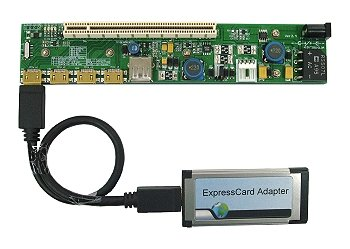
\includegraphics[width=0.75\columnwidth]{./pix/expresscard.jpg}\\
\end{center}

\end{document}

